\documentclass{article}
\usepackage[utf8]{inputenc}
\usepackage{graphicx}


%% pmateti: My changes are shown in comments like this.
% \usepackage{soul} % pmateti, check if overleaf has this pkg, and
% then uncomment
\usepackage[usenames,dvipsnames]{color}% pmateti
\newcommand\TBD{\textcolor{Red}{To Be Done~~}}% pmateti
\newcommand{\PM}[1]{\textcolor{Blue}{pmateti: #1}}% pmateti
\usepackage{url}                                  % pmateti
%% \newcommand\url{\texttt}        % pmateti if url pkg is unavailable
\usepackage{hyperref}           % pmateti

\begin{document}

\title{Cloud Storage Mounting on Android OS}
\author{Hanen Alkhafaji \\ \url{alkhafaji.2@wright.edu} \\ U00538764 \\ w004hba}
\date{June 8, 2019}
\maketitle


\begin{abstract}                % pmateti
This lab is intended to expose the user to the OCaml programming
language and the OCamlFUSE project available on GitHub. There are
familiarization tasks for the programming language, exploration tasks
for the open source code of OCamlFUSE, and tasks for mounting a Google
Drive storage on a Linux machine using OCamlFUSE.

\PM{Well done! ~~ \today}
\end{abstract}

\tableofcontents                % pmateti

\section{Objectives}

\begin{enumerate}
     \item Get comfortable with the OCaml programming language
     \item Get comfortable with the OCamlFUSE source code
     \item Successfully mount a Google Drive storage on a Linux machine using OCamlFUSE
\end{enumerate}

\section{Lab Experiment}

%% pmateti

\PM{Describe each task.\footnote{In the courses, we had a Lab Assignment
  written up.}
Use subsections, and subsubsections.}

\subsection{Task 1: Online OCaml Lessons}

\subsubsection{Simple Expressions} % pmateti
\subsubsection{Imperative Programming}
\subsubsection{Functions}
\subsubsection{New Examples by Hanen}
\subsubsection{Critique by Hanen}

\begin{enumerate}
\item Lesson 1 - Simple Expressions 
  This covered computing numeric values, defining strings, working with arrays, string manipulation, and defining and operating on tuples. Tuples can be made up of different data types. There are some functions built-in for tuples that have two elements. The functions presented in the tutorial were \texttt{fst} for getting the first element and \texttt{snd} for getting the second.

\item Lesson 2 - Imperative Programming 
  \texttt{let} is the keyword used to set the results of some computation to a named variable. However, once a variable is set to a particular value using the \texttt{let} keyword, it cannot be modified to a different value. A compilation error results. The way to get around this constraint is to use the keyword \texttt{ref} on the right side of the \texttt{let} statement. That reference can then be modified. (\texttt{let x = ref 42;;}) 
  \texttt{printf} is used similar to C to print formatted text to the terminal. 
  Looping syntax is very similar to many other program languages, except when looping through a series of numbers backwards the word \texttt{downto} is used as opposed to \texttt{to} in the ascending direction. 
  For comparison of values, the output is a boolean of either \texttt{true} or \texttt{false}. These greater than, less than, equal, or not equal to comparisons are not limited to only numeric values. The equal and not equal comparison symbols are similar to VB where a single equal sign represents an equivalence comparison while a less than sign followed by a greater than sign represents a non-equivalence comparison. The only limitation is that there isn't support for comparing values of different types. However, functions like \verb|string_of_int| can be used to convert an integer to a string so that it can be safely compared to another string. 
  \texttt{if then else} logic is very straight forward. 
  \texttt{while} loops logic is also easy to understand and uses a \texttt{while do done} structure.
\item Lesson 3 - Functions Functions can be defined in one line
  \PM{Huh?} using the \texttt{let} keyword very similar to defining a
  variable, but it takes arguments. One argument can be provided or
  several arguments in a tuple. Calling these functions is exactly the
  same as all other programming languages. Multiple values can be
  returned from a function by returning a tuple.  Defined functions
  can also be called in a partial manner. This almost seems like
  extension methods from the C\# world. A function that takes two
  arguments can be called with only one argument. However, it takes
  into account the value present at the time in which its called and
  uses that as the second parameter.  \texttt{let mul x y = x * y
    \\ let double = mul 2 \\ double 8} Anonymous functions are lambda
  expressions. They are functions defined without a name. These are
  useful for generating inline functions to be passed as a parameter
  to a function. In this case, they do not need to be assigned an
  identifier.  Functions such as \texttt{List.map} and
  \verb|List.fold_left| are useful for combining the power of
  anonymous functions and iterators to get a task done efficiently by
  iterating over a list and performing an operation on each value as
  the iterator visits each element.
\item
  \PM{A couple of new examples of OCaml by Hanen?}
\end{enumerate}

\PM{Give a brief opinion on the tutorial.}

\subsection{Task 2: Adjust OCaml Example Projects}
\subsubsection{Go Fish}
\begin{enumerate}
\item Original Source Code - I found the code for this game on Rosetta Code under the OCaml implementation. The game play is based on one player and an AI player who is automated through the back-end randomization functionality. The user chooses a card and asks the AI player if it has that card. If the AI player does, then it must give it. If the AI player does not, then the user must pick up a card from the deck. The player who loses their entire hand of cards first wins. As the code is currently written, the players are named "a" and "b". There is not a way to change that. Also, the user picks the card to ask about by typing in a number between a provided range which corresponds to the cards left in the player's hand.
\item Allowing For Choosing Players' Names - After wrestling with the code and trying to better familiarize myself with OCaml, this ended up being a pretty straight forward task. It took much longer since I made several failed attempts along the way trying to understand how OCaml projects are structured. The following code ended up being the only piece I needed to change. \\ \\
From this:
\begin{verbatim}
  (try
    if Random.bool()
        then make_turn "a" "b" player_a player_b
        else make_turn "b" "a" player_b player_a;
  with Exit -> ());
\end{verbatim}

To this:
\begin{verbatim}
  (try
    if Random.bool()
        then make_turn Sys.argv.(1) Sys.argv.(2) player_a player_b
        else make_turn Sys.argv.(2) Sys.argv.(1) player_b player_a;
  with Exit -> ());
\end{verbatim}

This is how it was executed through the terminal:
\begin{verbatim}
hanen@hanen:~/Desktop/gofish$ ocamlc -g -o gofish gofish.ml
File "gofish.ml", line 153, characters 21-36:
Warning 52: Code should not depend on the actual values of
this constructor's arguments. They are only for information
and may change in future versions. (See manual section 9.5)
\end{verbatim}

This is a snippet of the game-play:
\begin{verbatim}
hanen@hanen:~/Desktop/gofish$ ./gofish "dr. mateti" "hanen"

player hanen asked for Sixs
player dr. mateti gives (Six-Clubs)

player hanen asked for Fours
player dr. mateti has no Fours

(Queen-Clubs), (Jack-Clubs), (Nine-Spades), (Eight-Diamonds), 
(Nine-Hearts), (Nine-Clubs), (Queen-Spades), (Queen-Diamonds)
Ranks: Eight, Nine, Jack, Queen
choose from 1 to 4
\end{verbatim}
\end{enumerate}

\subsubsection{Guess the Number}
\begin{enumerate}
\item Original Source Code - The game-play on this Guess the Number game is very simple. A random number generator is used to "think of a number" and the player puts in numbers until they guess the number that was chosen at random. The user cannot specify the maximum of the range and they are not given any feedback on how far off they are from the selected number. \\ \\
The following is the current state of the code:
\begin{verbatim}
#!/usr/bin/env ocaml
 
let () =
  Random.self_init();
  let n =
    if Random.bool () then
      let n = 2 + Random.int 8 in
      print_endline "Please guess a number between 1 and 10 excluded";
      (n)
    else
      let n = 1 + Random.int 10 in
      print_endline "Please guess a number between 1 and 10 included";
      (n)
  in
  while read_int () <> n do
    print_endline "The guess was wrong! Please try again!"
  done;
  print_endline "Well guessed!"
\end{verbatim}

The following is the current game-play in the terminal:
\begin{verbatim}
hanen@hanen:~/Desktop/gofish$ ocamlc -g -o guessnum guessnum.ml
hanen@hanen:~/Desktop/gofish$ ./guessnum
Please guess a number between 1 and 10 excluded
1
The guess was wrong! Please try again!
2
The guess was wrong! Please try again!
3
The guess was wrong! Please try again!
4
The guess was wrong! Please try again!
5
The guess was wrong! Please try again!
6
Well guessed!
\end{verbatim}

\item Let User Specify Max of Range - I wanted to give the user the ability to specify what the max of the range should be for the number that is selected randomly for guessing. \\ \\
The following is the new state of the code after the adjustment:
\begin{verbatim}
let () =
  Random.self_init();
  let n =
    if Random.bool () then
      let n = 2 + Random.int ((int_of_string Sys.argv.(1)) - 2) in
      Printf.printf "Please guess a number between 1 and %s excluded \n" Sys.argv.(1);
      (n)
    else
      let n = 1 + Random.int (int_of_string Sys.argv.(1)) in
      Printf.printf "Please guess a number between 1 and %s included \n" Sys.argv.(1);
      (n)
  in
  while read_int () <> n do
    print_endline "The guess was wrong! Please try again!"
  done;
  print_endline "Well guessed!"
\end{verbatim}

The following is the new game-play in the terminal:
\begin{verbatim}
hanen@hanen:~/Desktop/gofish$ ocamlc -g -o guessnum guessnum.ml
hanen@hanen:~/Desktop/gofish$ ./guessnum 5
Please guess a number between 1 and 5 excluded 
2
The guess was wrong! Please try again!
3
Well guessed!
\end{verbatim}

\item Warm/Cold Indicator For Guess - I wanted to be able to implement in some logic that would let the user know if they are close or far off with their guess. Now that I'm allowing the user to choose any number for the max of the range, this is a nice-to-have feature. If they choose their max at 100, it would be helpful to know if they are close or not with their guess.
\end{enumerate}



\subsection{Task 3: Explore OCamlFUSE Source Code}

\texttt{(https://github.com/astrada/google-drive-ocamlfuse)}

\subsubsection{OCaml Development Environment}
\subsubsection{Study OCamlFUSE Source Code}

\begin{enumerate}
\item OCaml development environment \\ (https://github.com/janestreet/install-ocaml)
  \begin{enumerate}
  \item Install opam \\
    \texttt{sudo add-apt-repository ppa:avsm/ppa \\sudo apt update \\sudo apt install -y opam m4} 
    This was a success!
  \item Initialize opam\\ 
    \verb|sudo opam init -y --compiler=4.07.1| 
    \verb|sudo opam update -uy| 
    \verb|sudo echo $(opam env)| 
    This was a success!
  \item Install libraries and tools 
    \verb|sudo opam install -y async core js_of_ocaml js_of_ocaml-ppx| \\ \verb|merlin utop ocp-indent| 
    This installed so many things and took a while, but was a success!
  \item Test Installation
\begin{verbatim}
  hanen@hanen:~$ git clone https://github.com/janestreet/install-ocaml 
  Cloning into 'install-ocaml'...
  remote: Enumerating objects: 20, done.
  remote: Counting objects: 100% (20/20), done.
  remote: Compressing objects: 100% (14/14), done.
  remote: Total 58 (delta 10), reused 14 (delta 6), pack-reused 38
  Unpacking objects: 100% (58/58), done.
  hanen@hanen:~$ cd install-ocaml/01-hello-world
  hanen@hanen:~/install-ocaml/01-hello-world$ dune build hello_world.exe
  hanen@hanen:~/install-ocaml/01-hello-world$ dune exec ./hello_world.exe
  Hello, World
\end{verbatim}
\item Run Tests
\begin{verbatim}
  hanen@hanen:~/install-ocaml/01-hello-world$ 
  cd ../02-expect-tests
  hanen@hanen:~/install-ocaml/02-expect-tests$ 
  dune runtest
  Done: 17/19 (jobs: 1)File "expect_test_example.ml", 
  line 1, characters 0-0:
  diff (internal) (exit 1)
  (cd _build/default && /usr/bin/diff -u 
  expect_test_example.ml expect_test_example.ml.corrected)
  --- expect_test_example.ml      2019-06-08 15:37:18.946700012 
  -0400
  +++ expect_test_example.ml.corrected    2019-06-08 15:37:21.494597583 
  -0400
  @@ -2,5 +2,5 @@
  
  let%expect_test _ =
  let () = printf "foo" in
  -  [%expect {| bar |}]
    +  [%expect {| foo |}]
      ;;
\end{verbatim}
The test failed because there is a different in the actual results versus what was expected. The following commands will copy the results into what was expected and show that the tests will pass after that because there will no longer be a difference. 
\begin{verbatim}
  hanen@hanen:~/install-ocaml/02-expect-tests$ dune promote
  Promoting _build/default/expect_test_example.ml.corrected to 
  expect_test_example.ml.
  hanen@hanen:~/install-ocaml/02-expect-tests$ dune runtest
  hanen@hanen:~/install-ocaml/02-expect-tests$ git diff
  diff --git a/02-expect-tests/expect_test_example.ml b/
  02-expect-tests/expect_test_example.ml
  index 75a19d9..9bb1c70 100644
  --- a/02-expect-tests/expect_test_example.ml
  +++ b/02-expect-tests/expect_test_example.ml
  @@ -2,5 +2,5 @@ open! Core
  
  let%expect_test _ =
  let () = printf "foo" in
  -  [%expect {| bar |}]
    +  [%expect {| foo |}]
      ;;
\end{verbatim}
\item Editor Setup: Installed Visual Studio Code.  Install a plugin
  for OCaml through Visual Studio Code by opening Visual Studio Code,
  pressing Ctrl+P, and entering \texttt{ext install
    hackwaly.ocaml}\footnote{Insert citation.} into the text
  field. Once enter is pressed, Visual Studio code will automatically
  install the OCaml plugin.
  \end{enumerate}
\end{enumerate}
\begin{enumerate}

\item Study OCamlFUSE source code %% pmateti \item Review OCamlFUSE
  source code I downloaded the source code from GitHub
  (https://github.com/astrada/google-drive-ocamlfuse) and opened it in
  Visual Studio Code.
  \begin{enumerate}
  \item ML versus MLI file The first thing I noticed was that there
    were duplicate files in the source folder that simply had
    different extensions. After some research, I found that the
    extension ML stands for Meta Language which is the umbrella
    programming language that contains OCaml. I suspect that the
    extension MLI stands for Meta Language Interface, but I cannot be
    certain of that since I was unable to find its expansion in my
    research. The reason I suspect it is Interface is because of what
    I observed when I looked at the files themselves.  I opened
    bufferPool.ml and bufferPool.mli and compared them to each
    other. In the ML file, I found full function implementations while
    in the MLI file, I found a listing of function signatures. So, the
    MLI files must be interfaces that are used by other classes so as
    to hide the implementation in the ML from outsiders.  \PM{Compiled
      from ML to MLI.}

  \item Code Exploration
    \begin{enumerate}
    \item There is a Make module in the concurrentGlobal file. 
    \item The file drive.ml appears to have the bulk of logic behind
      this implementation.
    \item I picked a function from the buffer.mli interface file
      called \verb|write_to_block| and did a project wide search for
      it. I found it referenced in the drive.ml file as
      \\ \verb|Buffering.MemoryBuffers.write_to_block| I do not
      understand why the case is different in the reference. Buffering
      when calling the function versus buffering in the definition of
      the file. I would not have made that connection before, but now
      am aware of it.
    \item Gapi shows up all over the code. It stands for Google API.
    \end{enumerate}
  \end{enumerate}
\end{enumerate}

\PM{Study OCamlFUSE source code: Study every file.  Also, include sloccount.}

\subsection{Task 4: Mount Google Drive}
\subsubsection{Install OCamlFUSE}
\subsubsection{Allow Permissions through Browser }
\subsubsection{Make Directory and Mount Drive}

\begin{enumerate}
\item Run commands to install OCamlFUSE
\begin{verbatim}
  sudo add-apt-repository ppa:alessandro-strada/ppa
  sudo apt-get-update
  sudo apt-get install google-drive-ocamlfuse
  sudo google-drive-ocamlfuse
\end{verbatim}
\item Allow Permissions through Browser 
  Allow gdfuse to see, edit, create, and delete all of your Google Drive files. 
  Select Google account and allow access permissions.
  \begin{figure}[htb]
    \centering
    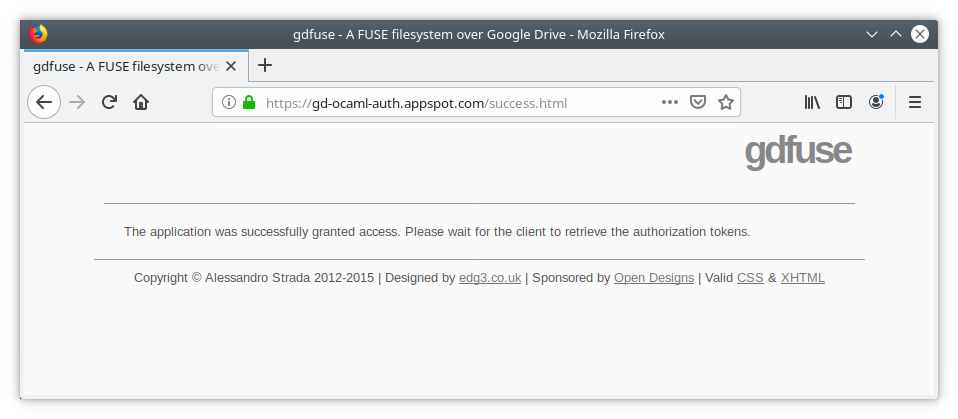
\includegraphics[scale=0.47]{ocaml7.png}
    \caption{Screenshot ocaml7.png}        % pmateti
    \label{fig:ocaml7}
  \end{figure}
\item Make Directory and Mount Drive
\begin{verbatim}
  hanen@hanen:mkdir ~/GoogleDrive
  hanen@hanen:google-drive-ocamlfuse ~/GoogleDrive
  hanen@hanen:cd GoogleDrive
  hanen@hanen:ls
  '2019-Hanen-CS 6970'    Misc
\end{verbatim}
That final output matches the contents of that Google Drive in the
browser as seen below.  \PM{Placement of figures is not quite in our
  control.  So we must refer to afig by its number.}  See Figure
\ref{fig:ocaml10}
\begin{figure}[htb]
  \centering
  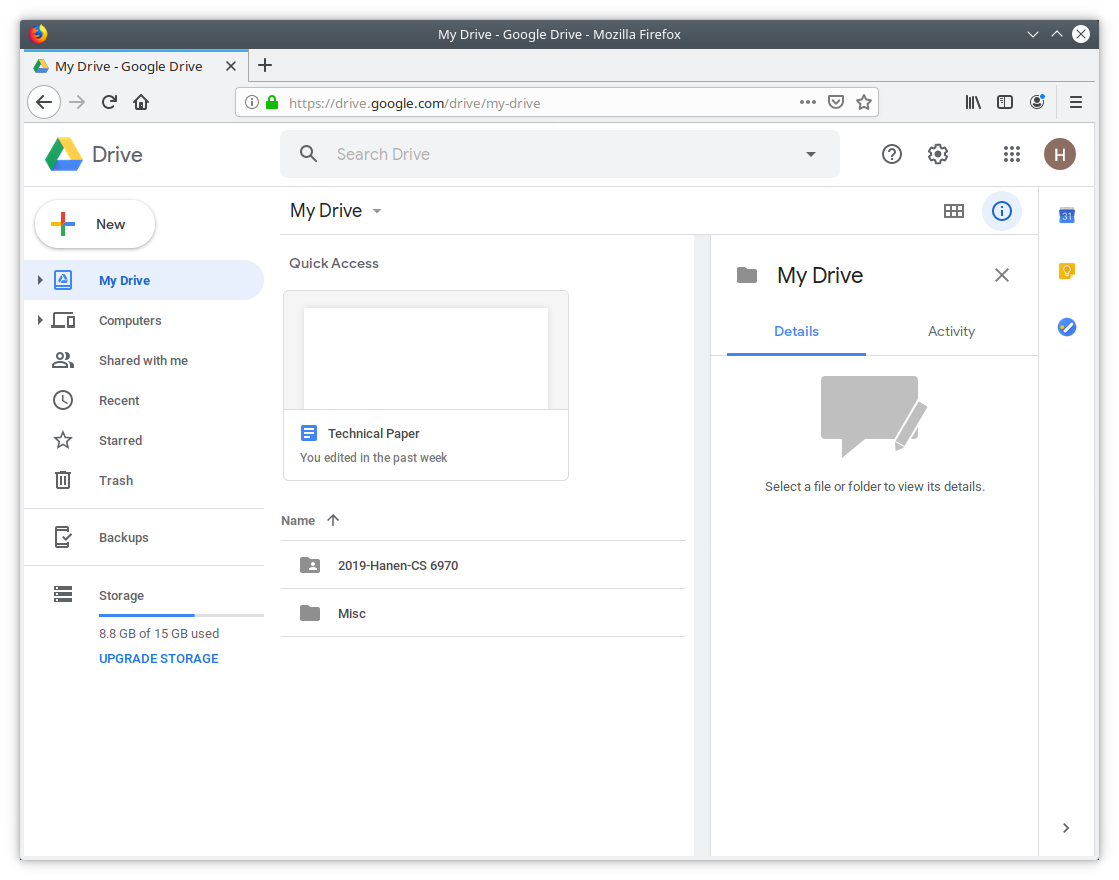
\includegraphics[scale=0.4]{ocaml10.png}
  \caption{Content of GD as seen through the browser} % pmateti
  \label{fig:ocaml10}
\end{figure}
\end{enumerate}

\section{Concluding Remarks}

\section{References}

\PM{We must have references.  Properly.  Author name, etc.  I did a
  highly incomplete job below.  Doing .bib can take an hour or two to
  learn -- so do it in a way that Overleaf suggests.}

\begin{description}
  \item [Example] Vangoor, Bharath Kumar Reddy, Vasily Tarasov, and
    Erez Zadok. ``To {FUSE} or Not to {FUSE}: Performance of User-Space
    File Systems.'' In 15th {USENIX} Conference on File and Storage
    Technologies ({FAST} 17), pp. 59-72. 2017. \href{https://www.usenix.org/system/files/conference/fast17/fast17-vangoor.pdf}{PDF}
  \item[OCaml Lessons] \url{https://try.ocamlpro.com/}
  \item[Source Code]
     \url{(https://github.com/astrada/google-drive-ocamlfuse)}
  \item[Rosetta Code: Go Fish] \url{http://rosettacode.org/wiki/Go_Fish/OCaml}
\end{description}

\end{document}
